\chapter{Segmentation}

In this chapter will be segmentation described, listed some techniques.
After that level set method will be described along with its relation to segmentation as well as computation issues. //TODO

\section{Problem formulation}
Segmentation is process when pixels of input image are split into several subsets (partitions) based on their characteristics or computed properties, such as color, intensity, or texture.
Pixels within such partition then have similar features and compose some object in the image.

In more formal way it is a function that assign a segment to pixel:
\begin{equation}
S: S(p) = k
\end{equation}
where p $\in$ pixels of an image and k $\in$ set of segments

Segmentation is used in many domains such as medicine (locating organs, tumors, bones, ...), parsing images from satellite for maps (location buildings, roads, ...), machine vision (fingerprint recognition, face, eyes, or other features recognition).
Or such simple tool as well known "magic-stick" tool in popular graphics editing software (Photoshop, GIMP) that performs thresholding segmentation.

Although there were some attempts to find general-purpose segmentation solution, results were not satisfactory.
So there is not yet such general solution. Each domain needs extra approach how to perform the segmentation.
Some of them are not even fully automatic so they need assistance of operator (semi-autonomous approaches).
In this kind of segmentation, the user (operator) inputs some region and thus give a hint to the algorithm.
This is favorite approach in segmentation of structures (organs, etc.) on medical images.
An physician then plays the role of the operator because of his knowledge of images' content.
Some are autonomous but needs some a priory knowledge of some properties of segmented object.

Sometimes segmentation methods are performed on different resolutions and then combined together.
Which means solution from lower resolution is taken as another input (some criterion, etc.) for solution of higher resolution.

\section{Segmentation methods overview}

Segmentation methods can be divided into following basic categories:

\begin{enumerate}

  \item Clustering

  These methodes are used do cluster an image into N clusters.
They covers the entire image.
Two main subsets of methods are bottom-up and top-bottom.
The first one takes each pixel as separate cluster and then iterate joining these initial clusters (pixels) based on some criterion until there are N cluster in cluster set.
The second one pick N (randomly or heuristic based) chosen cluster centres.
And then repeats these two step until some convergence condition is met (e.g. no pixels change clusters): assign pixels to clusters based minimalisation of the variance between the pixel and the cluster centre and re-compute the cluster centres by averaging all of the pixels in the cluster.

  \item Histogram-based

  As first, histogram is computed from pixels of the image.
Then peaks and valleys in the histogram creates the clusters in the image.
Result can be refined by recursively repeated the process.
Recursion is stopped when no new more segments appears.

  \item Edge detection

  These methods segment an image based on its edges.
So core of such methodes is some edge-detection algorithm (Canny, Sobel, ...).
Discontinuities of found edges that form the segmented object must be overcome some other technique (i.e. based on distance among edges, when two edges are close to each other they are considered to form boundary of segmented object).

  \item Region growing

  This set of methods are very similar to flood-fill algorithm.
It takes a set of seed points and a segmented image.
Each seed point is something like pointer to segmented object on the image.
Seed points forms initial set of segments.
Then iteration through the neighbouring pixels of an segment is performed.
In every step of that iteration an neighbour pixel is compared with region - similarity function is calculated.
If it is similar enough, the pixel is added to the region.
  Method is highly noise sensitive.
The initial seeds can be misplaced due to the noise.
So there is another algorithm that is seedless.
It starts with a single pixel (region).
Its location does not significantly influence final result.
Then the iteration over neighbouring pixels are taken just as in seeded growing.
If it is different enough (some threshold value is applied), new segment is created.
  Particular approaches differs in definition of the similarity function.
While one group uses pixel's properties (intensity, colour) directly, another computes some statistical test and the candidate pixel is processed according the test was accepted or rejected.

  \item Graph partitioning

  This approach converts an image into a graph (pixels corresponds the vertices.
There is edge between every pair of pixels and edges are weighted with similarity function of the two connected pixels).
Then some graph algorithm that cuts off edges and thus partition the graph (image) is then run.
Popular algorithms of this category are random walker, minimum mean cut, minimum spanning tree-based algorithm, normalized cut, etc.

  \item Watershed transformation

  The watershed transformation considers the gradient magnitude of an image as a topographic surface.
Pixels having the highest gradient magnitude intensities (GMIs) correspond to watershed lines, which represent the region boundaries.
Water placed on any pixel enclosed by a common watershed line flows downhill to a common local intensity minimum (LMI).
Pixels draining to a common minimum form a catch basin, which represents a segment.

  \item Model based segmentation

  The main idea of this method is to describe segmented object statistically (construct a probabilistic model) explaining the variation of the shape of the object.
In segmentation phase is the model used to impose constraints as prior.
Searching for such model contains steps like: registration of the training examples to a common pose, probabilistic representation of the variation of the registered samples and statistical correspondence between the model and the image.

  \item  Neural networks segmentation

  Neural Network segmentation relies on processing small areas of an image using a neural network or a set of neural networks.
After such processing the decision-making mechanism marks the areas of an image accordingly to the category recognized by the neural network.
A type of network designed especially for this, is the Kohonen map.

  \item Level set

Is method that uses mathematical implicit model of an segmented object.
It is represented as an surface of level set (LS) function defined on volume.
Surface is then deformed with forces that are computed from segmented image resulting actual segmentation of the object.

Whole process can be illustrated in very similar way to flood-filling, see figure \ref{fg:flooding}.
Initial surface (e.g. simple circle, for 2D case, as a surface of a distance function from given point) is deformed with forces that has direction of surface normals.
When it approaches borders of the object propagation slows down.
On borders on the object propagation stops (forces are zero there).

\begin{figure}
    \centering
    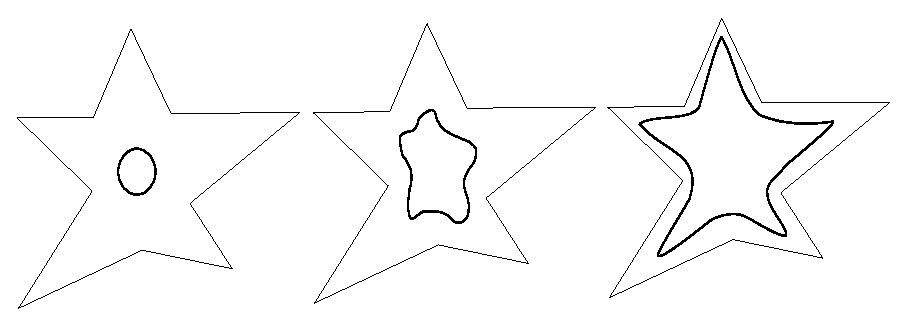
\includegraphics[width=12cm]{data/flooding}
    \caption[Flooding an object]{Initial shape (the circle) grows and fills (floods) the object on the background. In contrast to common flood-fill approach, level set method has several parameters that can e.g. prevent flooding beyond the object borders through small holes.}
    \label{fg:flooding}
\end{figure}

Another illustration uses landscape with a lake (in figure \ref{fg:shore}).
Water is always at constant altitude and the surface of an landscape changes in time.
With the changes of the landscape shoreline of the lake changes as well.
Landscape represents the LS function and water surface represent the surface i.e. k-level set.

\begin{figure}
    \centering
    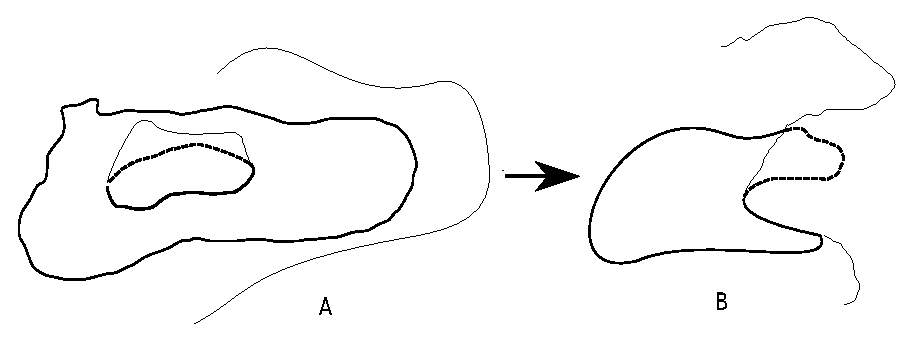
\includegraphics[width=15cm]{data/shore}
    \caption[Shore illustration of moving level set]{Picture A illustrates a lake with an island with a small rock on the right side. Level set is represent by the shore of that lake (thick line). As the level set moves it involves into picture B, the rock on the right suddenly grows to the left pushing the shoreline accordingly and make the island disappear.}
    \label{fg:shore}
\end{figure}

Advantages of the level set method is that it is implicit (no special stuff needed for merging and splitting surfaces), has only few intuitive parameters, can change the topology and can be performed in all dimension without explicit changes in method.

\end{enumerate}

\subsection{Level set formulation}

Level set method as proposed by Osher and Sethian \cite{sethianLS} provide numerical and mathematical mechanisms how to compute surface deformation as time varying iso-values of LS function using partial differential equations (PDE).
LS function is a signed scalar (distance) function
\begin{equation}
\phi : U_{x,y,z} \rightarrow \mathbb R,
\end{equation}
where $U \subset R^3$ is the domain of the volume (note: every definitions will be for 2D case).
$\phi$ can be sometimes called embedding. LS is implicit representation of an surface of the segmented object.
Surface is then subset of the LS function values
\begin{equation}
\vec{S} = \{\vec{x}\mid \phi(\vec{x}) = k\}
\end{equation}
S is then called an k-isosurface or k-level set of $\phi$. k can be chosen freely, but in most cases it is zero.
Surface is then called zero isosurface, zero LS or front in some contexts and corresponds to the actual object contour.

Surface can be also defined as local mapping $\vec{S}$:
\begin{equation}
\vec{S}: V_r \times V_s \rightarrow \mathbb R^3_{x,y,z},
\end{equation}
where $V \times V \subset \mathbb R^2$. Because of deformation time variable $t\in \mathbb R^+$ has to be added resulting function S = S(r,s,t).
Deformation (propagation) of the surface is then described by an evolution equation i.e. differential equation on S.
One approach (dynamic) is to use one-parameter family of $\phi$ i.e. $\phi(\vec{x},t)$ changes over time, $\vec{x}$ remains on the k-level set of $\phi$ as it moves and k remains constant.
Resulting equation is
\begin{equation}
\label{deformEq}
\phi(\vec{x}(t),t) = k \Rightarrow \frac{\delta \phi}{\delta t} = - \Delta \phi
\cdot \vec{v}.
\end{equation}
Where v represents movement of point x on deforming surface i.e. positions in time.
All surface movements depend on forces that are based on LS geometry.
And LS geometry can be expressed in terms of differential structure of $\phi$.
So following version of equation \ref{deformEq} link formulated:
\begin{equation}
\frac{\delta\phi}{\delta t} = - \Delta \phi \cdot \vec{v} = - \Delta \phi
\cdot F(\vec{x}, D\phi, D^2\phi, ...),
\end{equation}
where $D^n\phi$ is the set of n-order derivatives of $\phi$ evaluated at x.
The term $F(\vec{x}, D\phi, D^2\phi, ...)$ represents some force that influence the movement of a surface point.
This equation can applies to every values of k i.e. every LS of function $\phi$ and is basic equation of LS method.

\subsection{Level set computation}

Computation of surface deformation has to be discretized. So it is performed on discretized volume i.e. grid.
Equation converts the problem to solving nonlinear partial differential equations (PDE).
Surface deformation (propagation, movement) is then computed from initial model in cycles representing discrete time steps using this update equation:
\begin{equation}
\label{deformEqApprox}
\phi_{i,j,k}^{n+1} = \phi_{i,j,k}^{n} + \Delta t \Delta \phi_{i,j,k}^{n},
\end{equation}
where the term $\phi_{i,j,k}^{n}$ is discrete approximation of $\frac{\delta\phi}{\delta t}$ refering to the n-th time step at discrete position i,j,k (which has an counter part in continuous domain $\phi(x_i, y_j, z_k)$ ) and $\Delta t \Delta \phi_{i,j,k}^{n}$ is finite forward difference term representing approximation of the forces influencing the LS (update term). The solution is then succession of steps where new solution is obtained as current solution plus update term.

Discretization of the LS solution brings two problems.
Fist one is need of stable and accurate numeric scheme for solving PDE equations.
This is solved by proposed 'upwind scheme' by Osher and Sethian\cite{sethianLS}.
The second one is high computational complexity caused by conversion surface problem into (one dimension higher) volume problem.
// TODO popsat narocnost
Some

\subsection{Speed-up approaches}

Because of computational burden of level set solving some speed-up approaches has been proposed.
They are useful only when only single level set is computed (that is the case of segmentation).
In that case us unnecessary compute solution for given time step over whole domain but only in those parts that are adjacent to the level set (in its neighbourhood).
The most known and used are Narrow Bands and Sparse Fields.

Narrow Bands (proposed by Adalsteinsson and Sethian \cite{sethianFastLS}) computes embedding only within narrow band (tube).
Remaining points are set constant to indicate that they are not in the tube.
When LS reach the border of the tube, new tube has to be recalculated based on current LS and new run of embedding computations are performed on this new tube until envolving LS reaches tube borders.

\begin{figure}
    \centering
    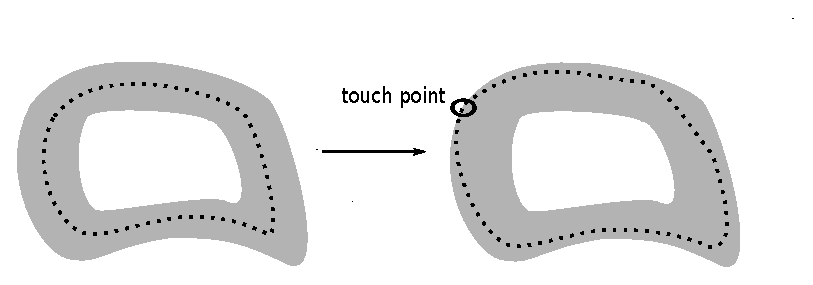
\includegraphics[width=\textwidth]{data/narrowBands}
    \caption[Narrow bands computation illustration]{Embedding computation is performed only within narrow band (highlighted in grey). When level set touches (highlighted by circle) the border or the band, new band has to be computed (reinitialized).}
    \label{fg:narrowBands}
\end{figure}

Sparse Fields method (proposed by Whitaker \cite{sparseFilelds}) introduces a scheme in which updates of an embedding are calculated only on the level set.
This means that it performs exactly the number of calculations that is needed to calculate next position of the level set.
This is the biggest advantage of the method. Points that are adjacent to the level set are called active points (forming active set).
Because active points must be adjacent to the LS their positions lie within certain range from the LS.
Therefore even values of an embedding in active set positions must lie on certain range (active range).
When active point value move out from this active range it is no longer the active point and is removed from the active set.
And vice versa, the point whose value comes into active range is added into active set.
Along the active set there is few layers of points adjacent to the active set organized like peels of an onion, see figure\ref{fg:sparseFilelds}.
Process can be imagined as a tram that lays down tracks before it and picks them up behind.

\begin{figure}
    \centering
    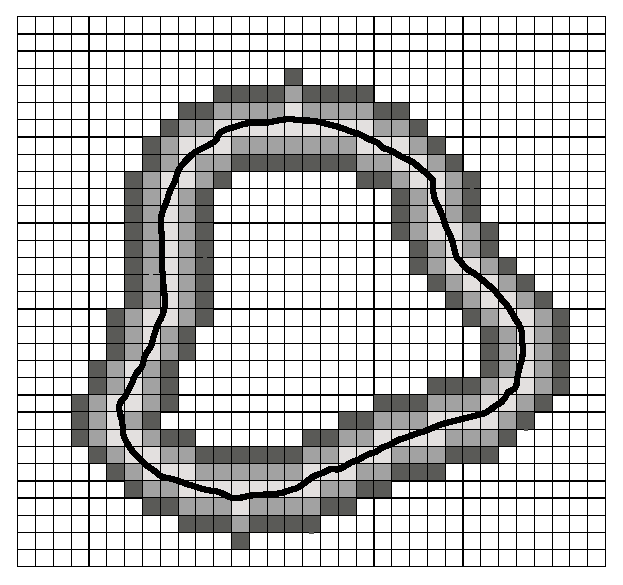
\includegraphics[width=\textwidth]{data/sparsefield}
    \caption[Sparse fields method computation illustration]{Embedding is calculated only at points that are covered by the level set (the white line). Those point (active set) are coloured in black forms the zero layer. Other layers embrace the zero layer from both inner and outer side, formed like onion peels}
    \label{fg:sparseFilelds}
\end{figure}


Algorithm:
\label{alg:sparseFileld}
1) FOREACH(point $\in$ active set (zero layer)
  a) compute level set geometry $\vec(x)$
  b) compute change using upwind scheme in point $\vec(x)$
2) FOREACH(point $\in$ active set compute new embedding value
$\phi_{i,j,k}^{n+1}$ (compute \ref{deformEqApprox}) and decide if it falls into
[-$\frac{1}{2}$,$\frac{1}{2}$] interval. If so, put the $\vec(x)$ into
appropriate status lists (list of points, that are changing status) to lower
status list if new value moved under the interval and vice versa.
3) Visit points in other layers $L_i$ in order $i=\pm 1,\ldots, \pm N$, and
update the values

//TODO

Even faster method that perform extension and distance reinitialization is $O(N)$ is presented by Peng et al. \cite{pengSparseFields}.

\subsection{Level set segmentation}

Segmentation using LS method is performed based on a speed function that is calculated from input (segmented image) and that encourages the mode to grow into direction where the object lies.
There are variety speed functions. In this work I use speed function based on threshold $T_{low}$ and $T_{hi}$ of the intensities from the input image.
If pixel has intensity value that is within the threshold interval (for maximum speed in the middle of threshold interval), the level set model grows (see figure \ref{fg:speedFunction}).
Otherwise it contracts as fast as the pixel has value further from the interval. The function $D$ is defined as:
\begin{equation}
\label{eq:speedFunction}
D(\vec{x}) =
\begin{cases}
V(\vec{x}) - T_{low} & \text{if $V(\vec{x}) < T_{mid}$}\\
T_{hi} - V(\vec{x}) & \text{if $V(\vec{x}) > T_{mid}$}\\
\end{cases}
\end{equation}
where $V(\vec{x})$ is pixel value in point $\vec{x}$ and $T_{mid}$ is the middle of the thresholding interval.

\begin{figure}
    \centering
    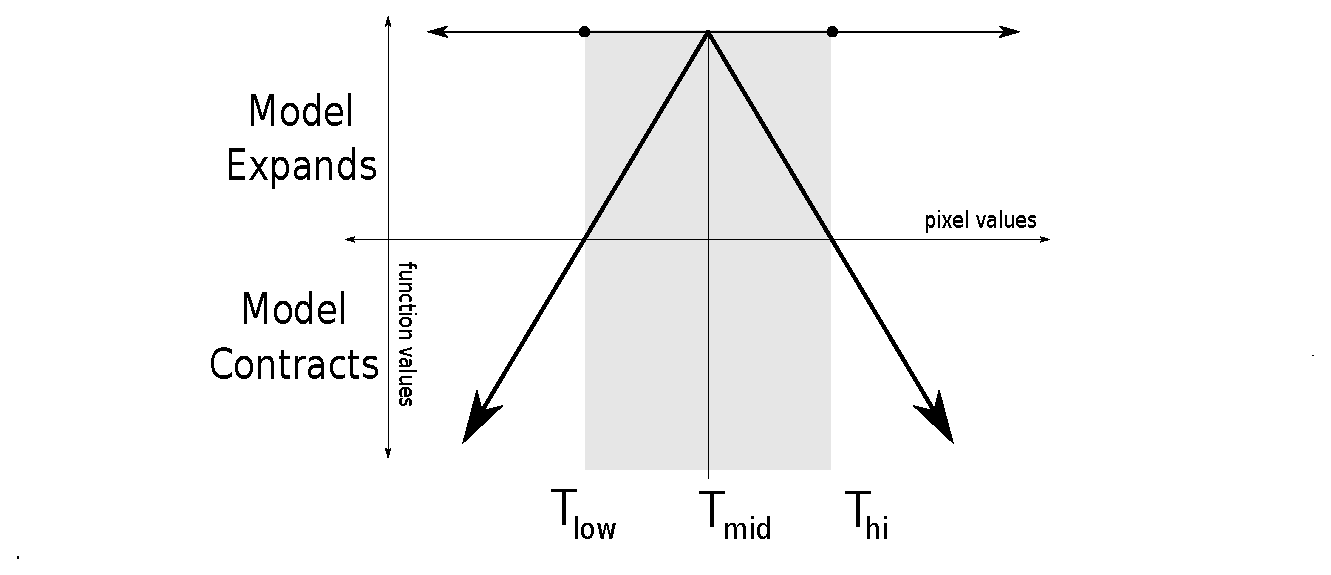
\includegraphics[width=\textwidth]{data/speedFunction}
    \caption[Graph of thresholding based speed function]{Gray rectangle encloses interval, where is the speed function positive (i.e. the model expands). The fastest expansion is in $T_{mid}$ point}
    \label{fg:speedFunction}
\end{figure}

This is quite natural definition of what we need from the process.
Grow as fast as possible where the segmented object lies and contract otherwise.

The update term from equation \ref{deformEqApprox} can be rewritten into following form that consist of few terms:
\begin{equation}
\phi_t = \alpha |\bigtriangledown \phi| H + \beta
\bigtriangledown|\bigtriangledown I|\cdot \bigtriangledown \phi +
\gamma|\bigtriangledown \phi|D
\end{equation}
where $|\bigtriangledown \phi|D$ represents speed function term, $\bigtriangledown|\bigtriangledown I|$ is edge term that is and $|\bigtriangledown \phi| H$ represent curvature term. $\alpha$, $\beta$ and $\gamma$ are weights of particular terms.

Edge term is computed from second order derivatives just like Canny and Marr-Hildreth algorithms for edge detection.
It shall to push level set towards edges (i.e. border of segmented object).

Curvature forces resulting level set model to have less surface and thus protect negative effects like levelset leaking into unwanted places like figure \ref{fg:leaking} shows.
Note: if $\alpha$ = $\beta$ = 0, the result is the same as from flood-fill method because there is only speed term taking place.

\begin{figure}
    \centering
    \includegraphics[width=\textwidth]{data/leaking}
    \caption[Leaking of segmentation into unwanted places]{}
    \label{fg:leaking}
\end{figure}

I omit the edge term so there is only two parameters of the method.
Tuning of the term weights has to be performed in order to have best results.

\section{Level set methods on streaming architectures}

\par
There was some attempts for mapping level set method onto special stream device.
There are some obstacles due to streaming architecture that has to be overcomed to efficiently solve the problem.
The first is that in order to take advantage streaming architecture, the streams of data must be large, contiguous blocks.
Thus the points in discrete grid near the level-set surface must be packed into data blocks that can be further processed by streaming processors.
Another difficulty is that the level set moves with each time step, and thus the packed representation must be quickly adapted.

\begin{figure}
    \centering
    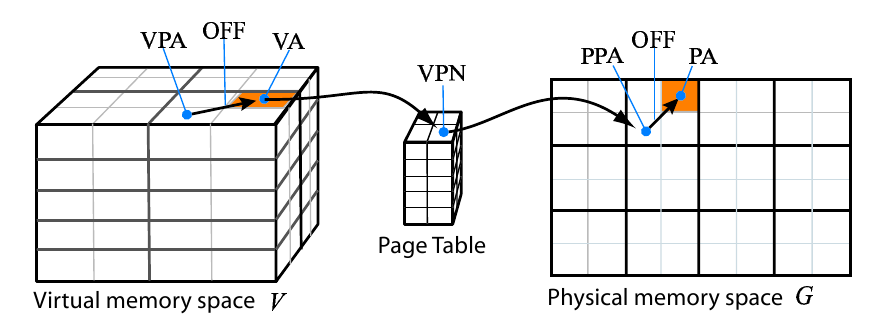
\includegraphics[width=\textwidth]{data/gpuVirtMemory}
    \caption[Leaking of segmentation into unwanted places]{}
    \label{fg:virtual memory on GPU}
\end{figure}

\par
For example Cates at al. \cite{GIST} or Lefohn at al. \cite{lefonhGPUSolver} mapped level set segmentation method onto GPU.
GPU is a streaming architecture with many (hundreds) of streaming cores. They runs short programs called shaders.
In mapping to GPU architecture texture memory is used to store input data (in large continuous block) and actual computation is managed by vertices that flows into the shader and plays role of some pointers to texture memory.
This is some kind of trick because the texture memory is not addressed directly by address number (like in single dimension continuous address space in common processors) but instead by a coordinate to texture.
So some virtual texture space has to be created like propose Lefonh at al. \cite{lefonhGPUSolver}.
Another workaround has to be performed when computed data is transferred back to CPU.
This direction is much more slower than CPU to GPU direction and thus the results has to be packed somehow.
Lefonh at al. \cite{lefonhGPUSolver} describes this packaging as well.
There are although some advantages.
One is the high count of the processors and extreme fast dedicated memory so the results can be impressive.
Another is that the calculation can be directly visualized by the GPU.

\par
Although Cell B.E. has some parts of the approach in common with GPU, such as streaming processors and thus need to pack the input data into larger continuous parts some GPU obstacles need not to overcome.
Its e.g. creation of virtual address space mapping coordinates to flat address space because the SPE directly has its own flat address space.
Also the result packing for sending back to CPU is not necessary because transmission of data from and to SPE has the same speed and can be performed directly.
All these Cell B.E. processor features could result easier and more straightforward process of mapping of level set method.
But probably at cost of lower speed than GPU.